% 2024本郷祭 マイコン部 部誌 「マイコンHONGOMagazine」 TeXテンプレート

% =環境設定=

\documentclass[b5paper,9pt,platex,dvipdfmx]{jsarticle}

% 数式
\usepackage{amsmath,amsfonts}
\usepackage{bm}

% 画像
\usepackage[dvipdfmx]{graphicx}
\usepackage{float}

% 段組
\usepackage{multicol}
\setlength{\columnseprule}{0.5pt}

\makeatletter
\def\mojiparline#1{
    \newcounter{mpl}
    \setcounter{mpl}{#1}
    \@tempdima=\linewidth
    \advance\@tempdima by-\value{mpl}zw
    \addtocounter{mpl}{-1}
    \divide\@tempdima by \value{mpl}
    \advance\kanjiskip by\@tempdima
    \advance\parindent by\@tempdima
}
\makeatother
\def\linesparpage#1{
    \baselineskip=\textheight
    \divide\baselineskip by #1
}

% 一行あたり文字数の指定
\mojiparline{20}
% 1ページあたり行数の指定
\linesparpage{45}

% 余白
\usepackage[paper=b5j,truedimen,margin=15truemm,dvipdfmx]{geometry}

% ページ番号を削除
\pagestyle{empty}

% ソースコード環境
\usepackage{listings,jlisting}
\lstset{
  basicstyle={\scriptsize\ttfamily},
  identifierstyle={\scriptsize},
  commentstyle={\smallitshape},
  keywordstyle={\scriptsize\bfseries},
  ndkeywordstyle={\scriptsize},
  stringstyle={\scriptsize\ttfamily},
  frame={tb},
  breaklines=true,
  columns=[l]{fullflexible},
  numbers=left,
  xrightmargin=1zw,
  xleftmargin=1zw,
  numberstyle={\scriptsize},
  stepnumber=1,
  numbersep=1zw,
  lineskip=0.5ex,
}
\renewcommand{\lstlistingname}{リスト}

% 枠付き文字(引用文)
\usepackage{fancybox}
\usepackage{ascmac}

% URL
\usepackage{url}

% ルビ
\usepackage{okumacro}

\usepackage{ulem}

% 書きたい内容に合わせてお好きなパッケージを導入していただいて構いませんが、外部パッケージは提出時に必ず合わせて提出してください。
% また、そのパッケージを使用している部分には必ずコメントをしてください。

% =環境設定ここまで=

\begin{document}

% =タイトル=
\title{Unityで文化祭用ゲームランチャーを作ろう}
\author{Wattz麻呂}
\date{\today}
\maketitle
% 初めのページのページ番号を削除(\maketitleの影響を回避)
\thispagestyle{empty}

% ここではページごとに段組しています。大きく画像を表示したいときなどは以下を \begin{multicols}{3} 、\end{multicols}のように変更すると文章が終わった直後から空白になります

% 以下本文
\begin{multicols}{3}
麻布の物理部無線班の部誌にUnityのコードエディターはVScodeみたいな事書かれてて憤慨しました。再びT.wattzです。(MacならわからんでもないけどWindowsならどっからどう考えてもVisualStudioですよねぇ(\#\textasciicircum$ \omega$\textasciicircum)\\
 それはさておき、AtsEXはニッチで複雑怪奇な話題だったのですが、今回はC\#プログラミングの定番であるUnityを使ってゲームランチャーを作っていきます!(半分筆者の日記みたいなものですが)\\
リポジトリはgithub.com/\\cydiawaltz/GameLuncher2024 にあるのでどうぞ御覧ください。Unityは2022.3.2f1が必要です。\\
あと、スクリプト内のところどころで括弧の付け方が気持ち悪いですが、紙面上の都合ですのでご了承ください。\\
%また無Asset主義者なので基本的にアセットは登場しないと思いますのでご安心下さい。\\
\\
まずはデザインを決めます。斯々然々でそこらへんに落ちてたPS2ソフト「ナムコミュージアム アーケードHits\verb|!|」をパクることに決定しました。(以下画像)\\
\begin{figure}[H]
  \centering
  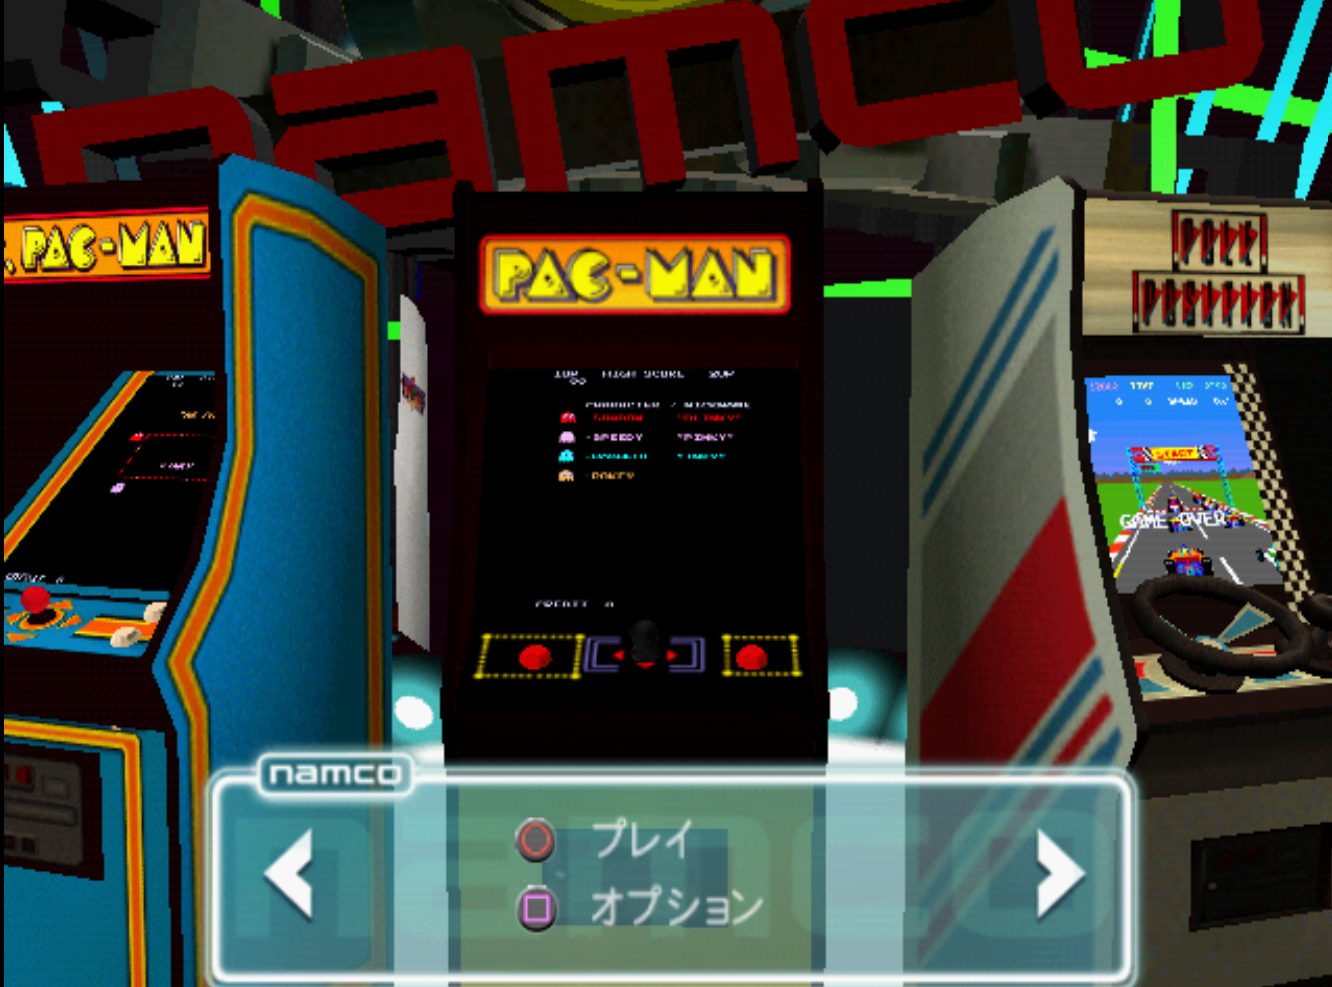
\includegraphics[width=5cm]{1.png}
  \caption{プライドなんてない。}
\end{figure}
よし。では早速Unityを開いてみましょう。そして、なんとなくいい感じにオブジェクトを配置します。\\
\begin{figure}[H]
  \centering
  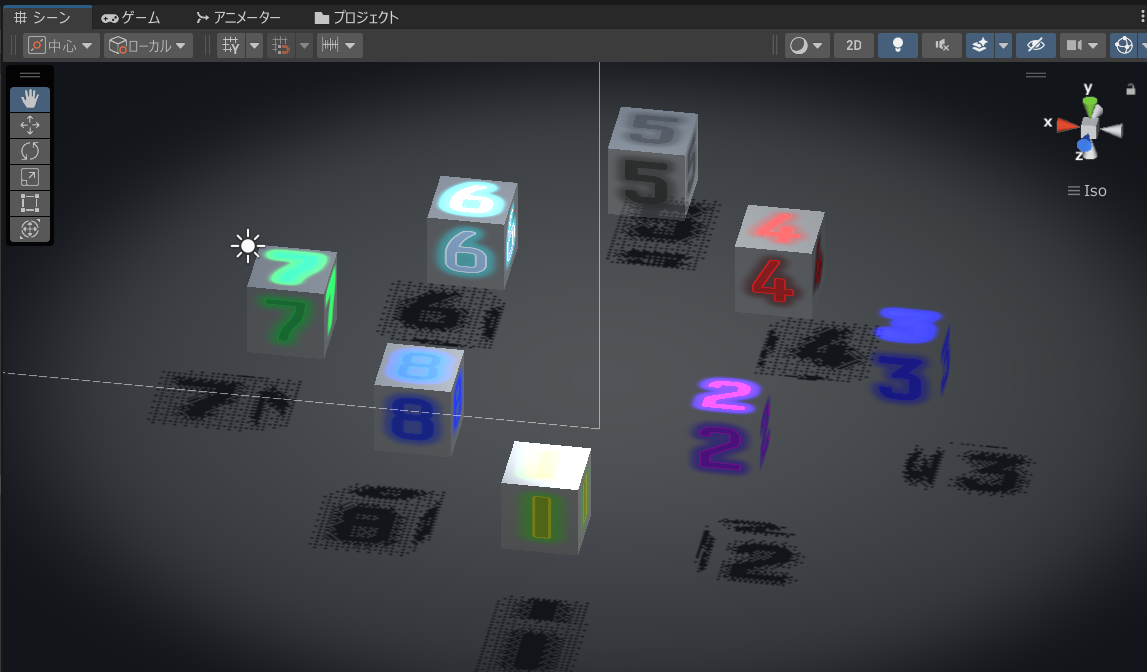
\includegraphics[width=5cm]{2.png}
  \caption{円状にオブジェクトを配置。}
\end{figure}
しました。では早速カメラを設置し、それを回すプログラムを記述しましょう。\\
\begin{figure}[H]
  \centering
  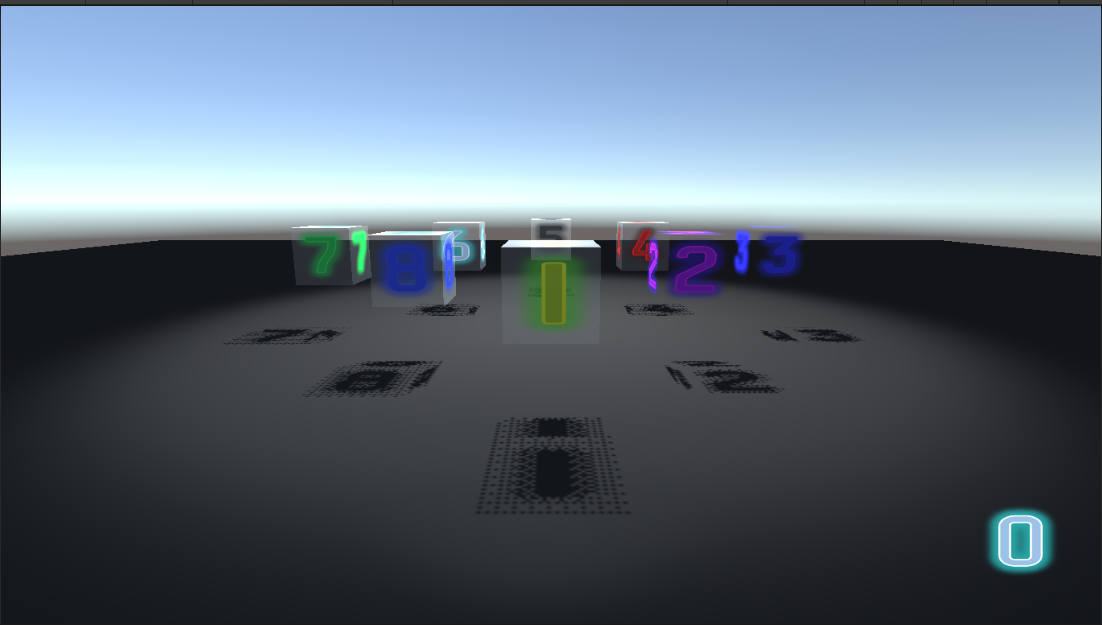
\includegraphics[width=5cm]{3.png}
  \caption{カメラを設置。}
\end{figure}
\begin{lstlisting}[caption=MoveNext.cs]
\\usingディレクティブ、クラス名とかは省略。
      public float speed;//移動する速度
      public int allObjects;//ゲームの総数
      public GameObject center;//回転の中心
      public int index;
      public int moveAngle;//回転角
      float moveSeconds;//回転する秒数
      public float currentAngle;//現在の角度
      void Start()
      {
          index = 1025;
          moveAngle = 360/allObjects;//回転角の大きさを設定
          moveSeconds = moveAngle/speed;//移動時間を設定
          currentAngle = 0f;//位置を初期化
      }
      void Update(){
          if(Input.GetKeyDown(KeyCode.RightArrow)){
              StartCoroutine(Move(-speed));
              index++;
              currentAngle = currentAngle+moveAngle;
          }
          if(Input.GetKeyDown(KeyCode.LeftArrow)){
              StartCoroutine(Move(speed));

              if(index == 0){SceneManager.LoadScene("HideScene");}//イースターエッグ
              else{index--;}
              currentAngle = currentAngle-moveAngle;
          }
      }
      public IEnumerator Move(float speed){
          float timer = 0f;
          while (timer < moveSeconds){
              transform.RotateAround(center.transform.position,new Vector3(0,1,0), speed);//これを唱えると第一引数(Vector3型)の位置を中心に回転します。
              //center.transform.positionは普通にVector3.zeroでいいです。
              timer ++;
              yield return null;
          }
      }
\end{lstlisting}
\end{multicols}
\begin{multicols*}{3}
(うわっ長っ、先が思いやられるなコレ)\\
このスクリプトを回転する物体(MainCamera)にアタッチし、インスペクタに諸々の情報を入力しましょう。\\
\begin{figure}[H]
  \centering
  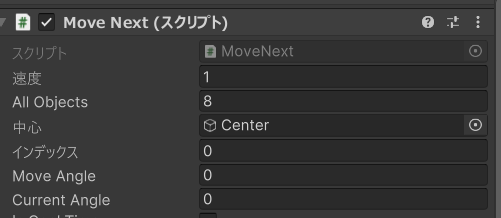
\includegraphics[width=5.5cm]{4.png}
  \caption{見にくっ。}
\end{figure}
これでオブジェクトを回転できました。へい。見づらいので紙版でご覧の方はpdf版で見るほうがいいかもしれません。まぁ、大したことやってる写真でもないのでシカトしてもらっても構いません。\\
次はUIにしましょうかねぇ。ではまたクソ長コードを御覧ください。\\
\begin{lstlisting}[caption=UIDraw.cs]
  public MoveNext moveNext;
  public int index;
  public bool isDisplay;//表示・非表示
  public GameObject imageObject;
  public Image imageComponent;
  public Sprite[] spriteImage;
  public GameObject buttonObject;
  public Image buttonComponent;
  public Sprite[] buttonImage;
  public GameObject info;
  void Start (){
      imageComponent = imageObject.GetComponent<Image>();
      buttonComponent = buttonObject.GetComponent<Image>();
      isDisplay = true;
  }
  void Update (){
      index = moveNext.index;
      if(isDisplay == true)
      {
          imageComponent.sprite = spriteImage[(index%(moveNext.allObjects))];//わりかし脳筋なのでspriteImage[0]にはallObjectsのをいれる
          buttonComponent.sprite = buttonImage[0];
          info.SetActive(true);
      }
      if(isDisplay == false)
      {
          buttonComponent.sprite = buttonImage[1];
          info.SetActive(false);
      }
  }
  public void OnClick (){
      isDisplay = !isDisplay;
  }
\end{lstlisting}
表示/非表示とスプライトの表示をまとめてみました。\\
同一オブジェクトのテクスチャ画像をindexの値に応じて変更する感じの処理です。\\
また、最後のメソッドOnclick()は表示/非表示を反転させるやつです。表示/非表示を入れ替えるボタンのOnClick()で呼び出します。\\
完成形はこんな感じになりま~す。\\
\begin{figure}[H]
  \centering
  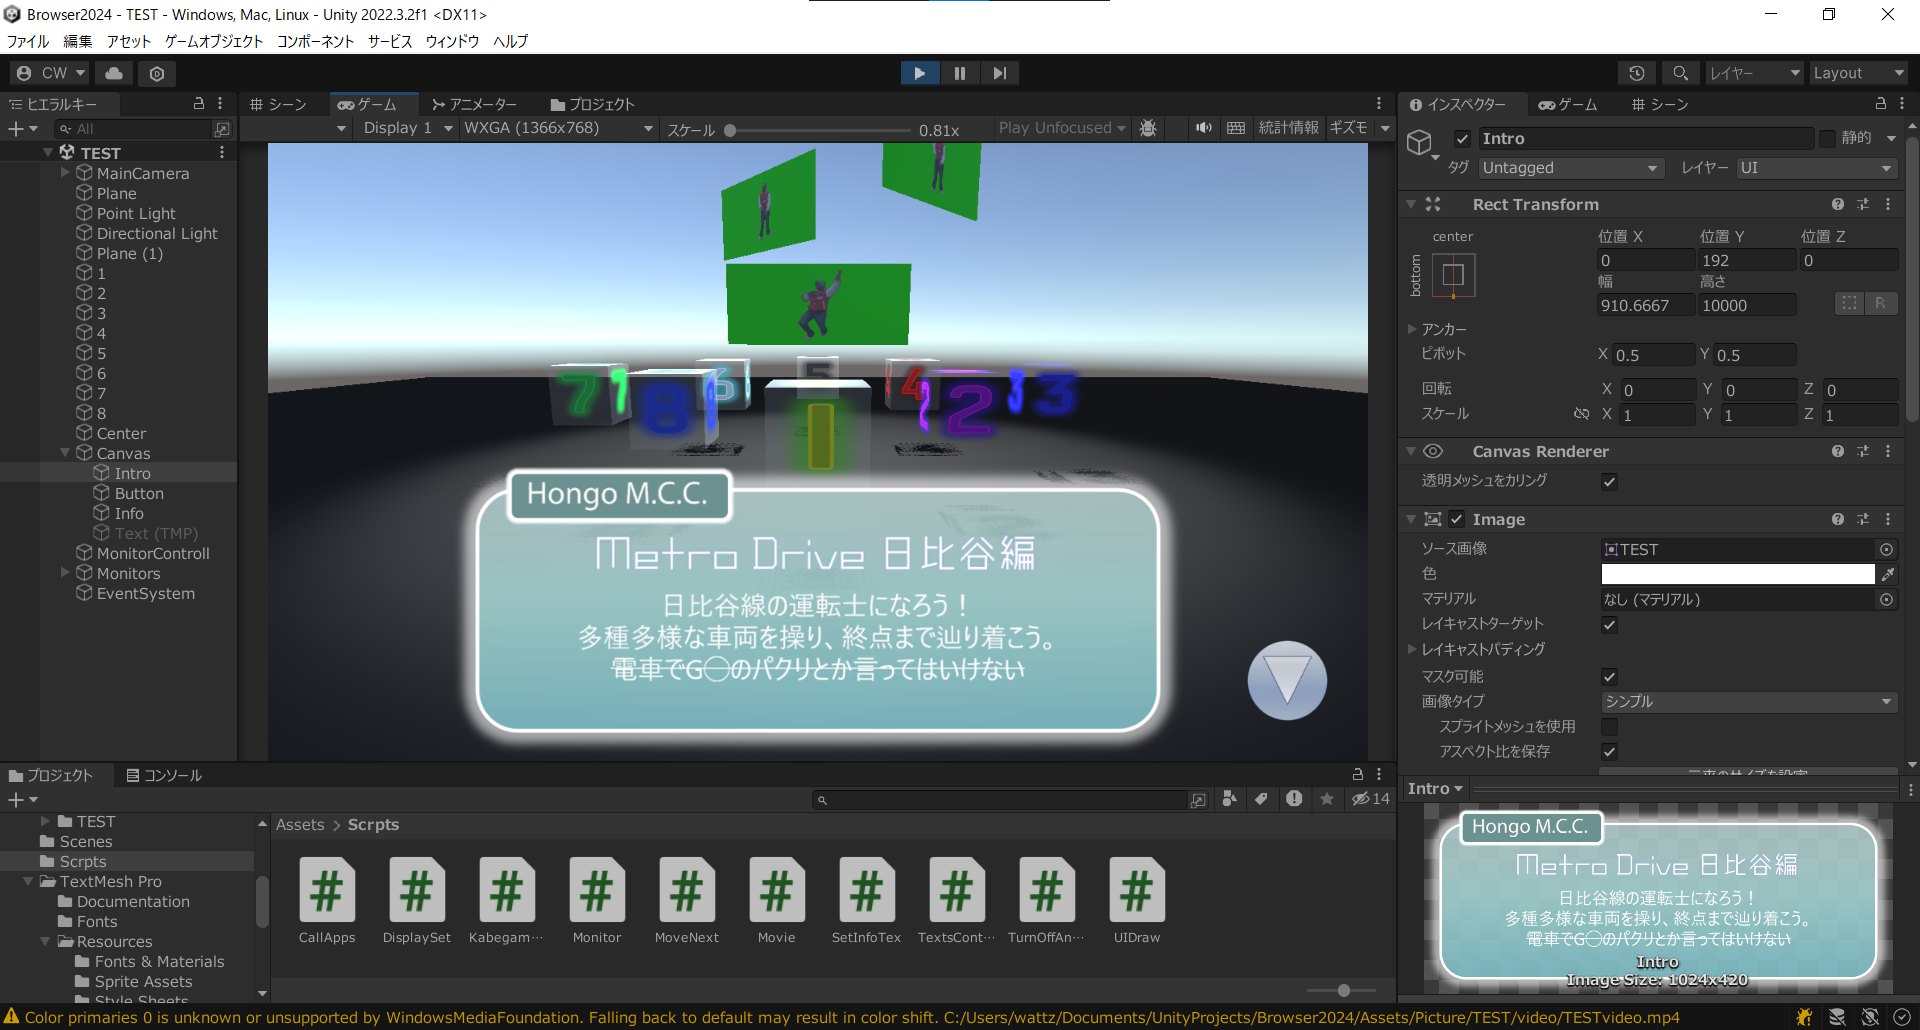
\includegraphics[width=5.5cm]{5.png}
  \caption{回転すると変わります。}
\end{figure}
\begin{figure}[H]
  \centering
  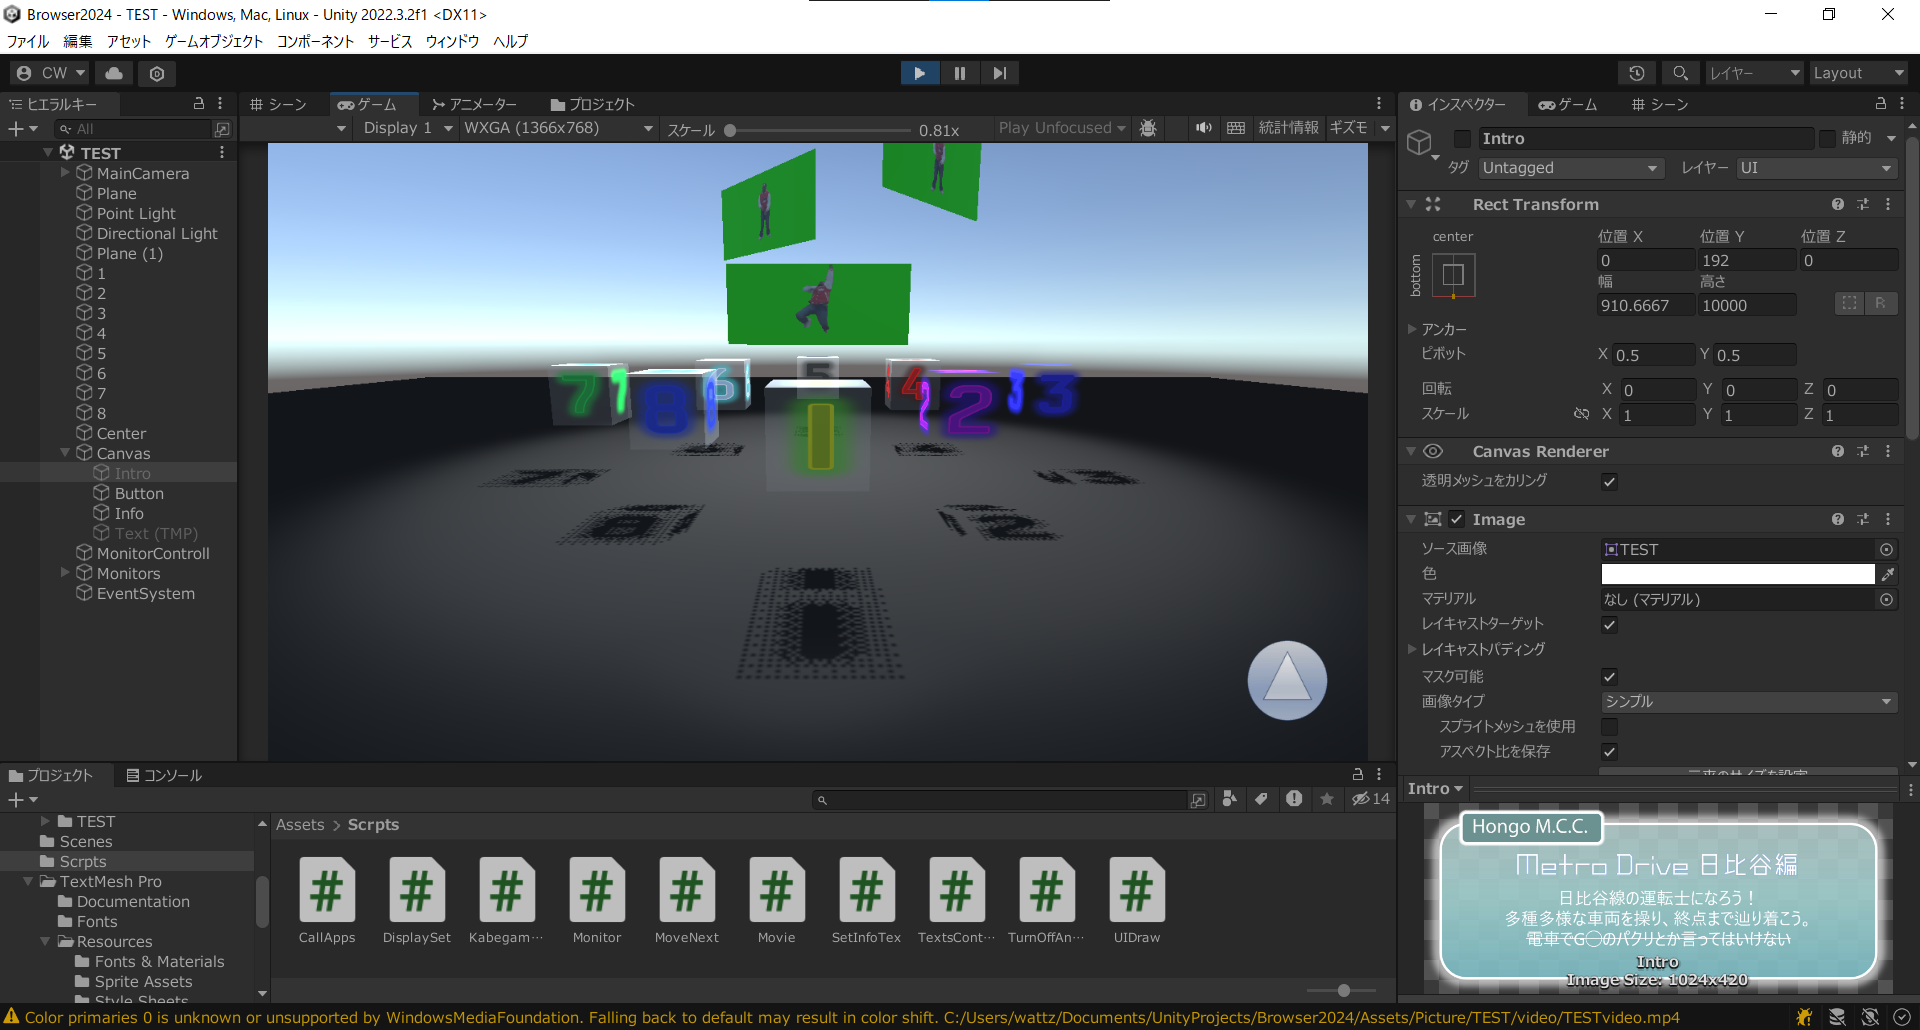
\includegraphics[width=5.5cm]{6.png}
  \caption{非表示にもできます。}
\end{figure}
次に解像度に応じて諸々を調整します。いらない?まぁ、ウインドウの大きさいじれるし、多少はね?\\
\begin{lstlisting}[caption=DisplaySet.cs]
  public float bairitu;//倍率に応じて画像の大きさを変更
  public bool isSetWidth;//縦に合わせる(インスペクターで選んでね♡)
  void Update()
  {
      int width = Screen.width;
      int height = Screen.height;
      RectTransform rectTransform = GetComponent<RectTransform>();//対象のオブジェクトにアタッチ
      if (isSetWidth){
          rectTransform.SetSizeWithCurrentAnchors(RectTransform.Axis.Horizontal, width / bairitu);
      }
      else{
          rectTransform.SetSizeWithCurrentAnchors(RectTransform.Axis.Vertical, height / bairitu);
      }
  }
\end{lstlisting}
うん。いい感じ。isSetWidthをtrueにしておくと横幅に、falseにすると縦幅に合うよう調整します。\\
bairituの値は現物合わせで調整しました。(解像度が1920*1080でisSetWidthをtrueにしてるとき、bairituが2だと1920/2=960で横幅は960pxに調整されます。)\\
次に位置。このままだと解像度が大きいほど下に下がってしまって遺憾なのでそれもスクリプトでゴリ押し。\\
\sout{今思ったけど普通にピポットを下部に}\\
\sout{調整すればよかっただけジャマイカ...?}\\
\begin{lstlisting}[caption=SetInfoTex.cs]
  RectTransform rectTransform;
  public int heightBairitu;
  void Start(){
      rectTransform = this.GetComponent<RectTransform>();
  }
  void Update(){
      int height = Screen.height;
      float posHeight = height / heightBairitu;
      rectTransform.anchoredPosition = new Vector2(0,posHeight);
  }
\end{lstlisting}
あんまり綺麗なコードじゃないですね...精進します。先ほどと同じように倍率の値を設定すると解像度に関わらずいい感じの見た目になります。\\
最後を\\new Vector2(this.transform.position\\.x,posHeight)\\
とするとxの値が毎フレームごとにどんどん増えていくんですよねぇ...なんでだろ。\\
UIも実装したので、メインディッシュであるアプリ起動の実装に移ります。\\
\begin{lstlisting}[caption=CallApps.cs]
  using UnityEngine;
  using System.Diagnostics;
  using System.IO;
  public class CallApps : MonoBehaviour{
      public MoveNext moveNext;
      public int index;
      public string exepath;
      public string readmePath;
      string type;
      public bool isHTML;
      public bool isNeedQuit;
      public int currentNum;
      private void Update(){
          index = moveNext.index%moveNext.allObjects;
          if(isHTML){ type = "html";}
          else { type = "exe"; }
          exepath = Path.Combine(Application.dataPath, "../Apps/GAME" + index + "/main." + type);
          readmePath = Path.Combine(Application.dataPath, "../Apps/GAME" + index + "/readme.txt");
          if (Input.GetKeyDown(KeyCode.Z)&&index == currentNum) {
            LaunchApp(isHTML, isNeedQuit);
          }
          if(Input.GetKeyDown(KeyCode.X)&&index == currentNum){
            LaunchReadMe();
          }
      }
      public void LaunchApp(bool isHTML,bool isNeedQuit){
          Process.Start(exepath);
          if(isNeedQuit == true) {
            Application.Quit();
          }
      }
      public void LaunchReadMe(){
        Process.Start(readmePath);
      }
  }
\end{lstlisting}
まあ簡単な実装ですが。一番の見どころはSystem.Diagnostics.Process.Start(string fileName)でしょうか。\\
これを呼び出すとファイルを開くことができます。便利。ちなみにProcessStartInfoってのを叩くと他にも引数を指定したりいろいろできるのですが、こちらについては今回あまり関係ないので割愛。(「MetroDrive 日比谷編」付属のコンポーネントインストーラも引数付きで起動してるのでサイレントインストールが使えてます。)\\
インスペクタからisNeedQuit(負荷の大きいゲームとかフルスクリーンのゲーム等でtrue)、isHTML(HTMLゲームでtrue)とかを設定します。起動は伝統に従ってZでアプリ起動としました。\\
半ページ残ってるのでプレイ画面の軽量化でもやりましょうか。\\
\begin{lstlisting}[caption=Monitor.cs]
  public GameObject[] monitors;//無計画な実装のせいで1から始まる
  public GameObject offMonitorsL;
  public GameObject offMonitorsR;
  public MoveNext moveNext;//MoveNext.cs
  public GameObject[] beginOffMonitor;//めんどくさいので最初に描画しないモニターは手動で設定したれ
  public int canSee;//表示されるモニターの値
  void Start(){
      monitors[(moveNext.index%moveNext.allObjects)].SetActive(true);
      canSee = (90 / moveNext.moveAngle);//横90°+1で開始時に白飛びするのを防止
      foreach(GameObject beginOff in beginOffMonitor){
          beginOff.SetActive(false);
      }
      foreach (GameObject monitor in monitors){
          monitor.GetComponent<VideoPlayer>().Pause();//全部開始時には一時停止
      }
      monitors[moveNext.index % moveNext.allObjects].GetComponent<VideoPlayer>().Play();
  }
  void Update(){
      if(Input.GetKeyDown(KeyCode.RightArrow)){
          monitors[((moveNext.index-canSee-1)%moveNext.allObjects)].SetActive(false);
          monitors[((moveNext.index+canSee)%moveNext.allObjects)].SetActive(true);
          foreach(GameObject monitor in monitors)//一旦全部オフにする
          {
              monitor.GetComponent<VideoPlayer>().Pause();
          }
          monitors[moveNext.index % moveNext.allObjects].GetComponent<VideoPlayer>().Play();//今表示されてるモニターだけOnにする
      }
      if (Input.GetKeyDown(KeyCode.LeftArrow)){
          monitors[((moveNext.index+canSee+1)%moveNext.allObjects)].SetActive(false);
          monitors[((moveNext.index-canSee)%moveNext.allObjects)].SetActive(true);
          foreach (GameObject monitor in monitors)
          {
              monitor.GetComponent<VideoPlayer>().Pause();
          }
          monitors[moveNext.index % moveNext.allObjects].GetComponent<VideoPlayer>().Play();
      }
  }
\end{lstlisting}
これで見えてるオブジェクトだけがSetActive(true)されるようになりました。満足。\\
他にもテクスチャ圧縮とかコライダーの削除とかで軽量化をいろいろ頑張りました。偉い。\\
あとはゲームです。さぁ、これが読まれているときにゲームはできているのでしょうか....\\
\begin{figure}[H]
  \centering
  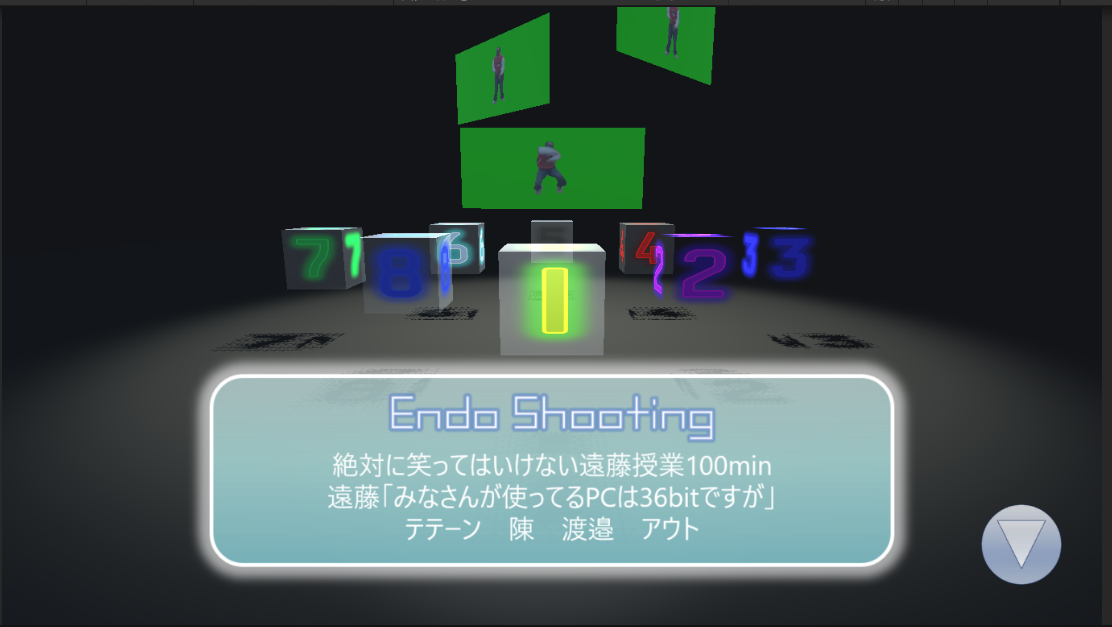
\includegraphics[width=5.5cm]{7.png}
  \caption{とりあえずテストは成功。}
\end{figure}
\end{multicols*}
% ソースコードを挿入するときは以下のようにしてください
%\begin{lstlisting}[caption=Sample]
%mes "hello, world!"
%\end{lstlisting}
%\end{multicols}
\end{document}